% =========================================================
%  Mini Proyecto 1 — Vectorizacion de un Kernel Numerico
%  Deteccion de Bordes con el Operador Prewitt
%  Programacion en Plataformas Multicore
%  Dr. Mario Rossainz Lopez — BUAP — 2026
% =========================================================
\documentclass[twocolumn,twoside]{Jornadas}

% ---- Codificacion y lenguaje ----
\usepackage[utf8]{inputenc}
\usepackage[T1]{fontenc}
\usepackage[spanish,es-nodecimaldot]{babel}

% ---- Matematicas ----
\usepackage{amsmath}
\usepackage{amssymb}

% ---- Graficos y figuras ----
\usepackage{graphicx}
\usepackage[caption=false,font=footnotesize]{subfig}
\usepackage{caption}
\captionsetup{font=footnotesize}

% ---- Tablas ----
\usepackage{booktabs}
\usepackage{array}

% ---- Flotantes (permitir mas figuras por pagina) ----
\setcounter{topnumber}{10}
\setcounter{bottomnumber}{10}
\setcounter{totalnumber}{10}
\renewcommand{\topfraction}{1}
\renewcommand{\bottomfraction}{1}
\renewcommand{\textfraction}{0}
\renewcommand{\floatpagefraction}{1}

% ---- Colores y codigo fuente ----
\usepackage[dvipsnames]{xcolor}
\usepackage{listings}
\definecolor{gray97}{gray}{.97}
\definecolor{gray75}{gray}{.75}
\definecolor{gray45}{gray}{.45}
\definecolor{codegreen}{rgb}{0,0.5,0}
\definecolor{codegray}{rgb}{0.4,0.4,0.4}
\definecolor{codeblue}{rgb}{0,0,0.6}

\lstset{
    inputencoding=utf8,
    extendedchars=true,
    backgroundcolor=\color{gray97},
    showstringspaces=false,
    basicstyle=\scriptsize\ttfamily,
    commentstyle=\itshape\color{codegreen},
    keywordstyle=\bfseries\color{codeblue},
    stringstyle=\color{gray45},
    linewidth=.98\columnwidth,
    xleftmargin=3mm,
    breaklines=true,
    numbers=left,
    numbersep=6pt,
    numberstyle=\tiny\color{codegray},
    firstnumber=1,
    frame=single,
    rulecolor=\color{gray75},
    escapeinside={(*@}{@*)},
    literate=
      {á}{\'a}1 {é}{\'e}1 {í}{\'\i}1 {ó}{\'o}1 {ú}{\'u}1
      {Á}{\'A}1 {É}{\'E}1 {Í}{\'I}1 {Ó}{\'O}1 {Ú}{\'U}1
      {ñ}{\~n}1 {Ñ}{\~N}1 {¿}{\textquestiondown}1 {¡}{\textexclamdown}1
}

% ---- Hiperenlaces ----
\usepackage{hyperref}
\usepackage{url}
\usepackage{placeins}

% ---- Ruta de figuras ----
\graphicspath{{./Figuras/}}

% ---- Separacion de silabas en espanol ----
\hyphenation{vec-to-ri-za-cion ren-di-mien-to pro-ce-sa-mien-to
             in-tri-se-cos in-ten-si-dad a-rit-me-ti-ca
             me-mo-ria com-pi-la-dor}

% =========================================================
%  METADATOS DEL DOCUMENTO
% =========================================================
\title{Vectorizaci\'on de un Kernel Num\'erico Aplicado a la\\
       Detecci\'on de Bordes en Im\'agenes y su An\'alisis\\
       de Rendimiento usando Intel Advisor}

\author{
  Alfonso P\'erez Garc\'ia%
  \thanks{Maestr\'ia en Sistemas Distribuidos,
          Benem\'erita Universidad Aut\'onoma de Puebla (BUAP),
          Puebla, Pue., M\'exico.}
}

% =========================================================
\begin{document}

\maketitle
\markboth{}{}
\pagestyle{empty}
\thispagestyle{empty}

% ---- Abstract ----
\begin{abstract}
Se presenta el an\'alisis de rendimiento de cuatro variantes de
vectorizaci\'on SIMD aplicadas a un kernel num\'erico de detecci\'on
de bordes mediante el operador Prewitt sobre im\'agenes en escala
de grises de 256$\times$256 p\'ixeles.
Las versiones implementadas son: escalar (sin vectorizaci\'on),
vectorizaci\'on autom\'atica del compilador Intel \texttt{icpx},
vectorizaci\'on guiada con \texttt{\#pragma omp simd simdlen(8)},
y vectorizaci\'on expl\'icita con intr\'insecos AVX2.
Los experimentos se ejecutaron con $N = 256 \times 256 \times 800 =
52{,}428{,}800$ operaciones para obtener mediciones estables.
El an\'alisis con Intel Advisor revela que el kernel es
\textit{memory-bound} con intensidad aritm\'etica te\'orica
$\mathcal{I} = 0.333$ FLOP/Byte, lo que limita las ganancias de
vectorizaci\'on a un m\'aximo de $1.24\times$ sobre la versi\'on escalar
(7.34 vs.\ 5.92~GFLOPS).
Los resultados muestran que el cuello de botella no es la capacidad
de c\'omputo SIMD, sino el ancho de banda de memoria disponible,
confirmado por la gr\'afica Roofline de Intel Advisor.
\end{abstract}

\begin{keywords}
  Vectorizaci\'on SIMD, Intel Advisor, operador Prewitt,
  detecci\'on de bordes, rendimiento HPC, AVX2, an\'alisis Roofline,
  \textit{memory-bound}.
\end{keywords}

% =========================================================
%  SECCIONES
% =========================================================
% =========================================================
%  SECCIÓN I — INTRODUCCIÓN
% =========================================================
\section{Introducci\'on}

\PARstart{L}{a} detecci\'on de bordes es una de las operaciones
fundamentales en el procesamiento digital de im\'agenes.
Su objetivo consiste en identificar los cambios abruptos en la
intensidad luminosa de los p\'ixeles de una imagen, los cuales
generalmente corresponden a las fronteras entre objetos, texturas
o regiones de inter\'es~\cite{gonzalez2008}.
Esta operaci\'on es el primer paso en cadenas de an\'alisis m\'as
complejas, como la segmentaci\'on sem\'antica, el reconocimiento
de objetos o la reconstrucci\'on tridimensional en aplicaciones
de visi\'on artificial, medicina, rob\'otica y teledetección
satelital~\cite{canny1986}.

El rendimiento de estas operaciones se vuelve cr\'itico cuando
se procesan grandes vol\'umenes de informaci\'on, como video en
tiempo real (30--60 cuadros por segundo), im\'agenes m\'edicas de
alta resoluci\'on (tomograf\'ia, resonancia magn\'etica) o flujos
de datos provenientes de sensores en sistemas embebidos.
Los procesadores modernos incorporan unidades de ejecuci\'on
vectorial (SIMD, \textit{Single Instruction, Multiple Data})
capaces de procesar m\'ultiples datos en paralelo dentro de un
\'unico n\'ucleo de c\'omputo.
En la arquitectura x86-64, la extensi\'on AVX2 (\textit{Advanced
Vector Extensions 2}) permite operar con registros YMM de 256~bits,
procesando hasta ocho valores de punto flotante simple
(32~bits) en una sola instrucci\'on~\cite{intel_intrinsics}.

Sin embargo, explotar correctamente la vectorizaci\'on SIMD no es
trivial.
El compilador puede vectorizar autom\'aticamente cuando detecta
patrones seguros, pero en ocasiones requiere ayuda mediante pragmas
o directivas.
Para m\'axima eficiencia, el programador puede emplear intr\'insecos
AVX2 directamente, aunque esto eleva la complejidad del c\'odigo.
Independientemente de la estrategia de vectorizaci\'on adoptada,
el rendimiento final puede estar limitado por el ancho de banda
de memoria del sistema, un fen\'omeno conocido como
\textit{memory-bound}~\cite{williams2009}.

El presente trabajo analiza estas cuatro estrategias aplicadas
al kernel num\'erico del operador Prewitt~\cite{gonzalez2008,prewitt1970}.
Se elige el operador Prewitt frente al Sobel por su estructura
con pesos uniformes ($\pm 1$), que produce una intensidad
aritm\'etica te\'orica reducida ($\mathcal{I} \approx 0.333$~FLOP/Byte)
y lo convierte en un candidato ideal para estudiar el
comportamiento \textit{memory-bound} en el modelo Roofline.
Se utiliza Intel Advisor como herramienta de perfilado para
obtener datos objetivos sobre intensidad aritm\'etica, modelo
Roofline y comportamiento de los bucles vectorizados.
La hip\'otesis de trabajo es que la intensidad aritm\'etica del
kernel ($\mathcal{I} \approx 0.333$ FLOP/Byte) situar\'a todas
las versiones en la zona de memoria limitada del modelo Roofline,
independientemente del nivel de vectorizaci\'on aplicado.

El resto del art\'iculo est\'a organizado de la siguiente manera:
la Secci\'on~II presenta el marco te\'orico sobre el operador
Prewitt, vectorizaci\'on SIMD e Intel Advisor;
la Secci\'on~III describe la metodolog\'ia experimental;
la Secci\'on~IV presenta los resultados obtenidos;
la Secci\'on~V discute e interpreta los datos;
y la Secci\'on~VI expone las conclusiones del trabajo.

% =========================================================
%  SECCIÓN II — MARCO TEÓRICO
% =========================================================
\section{Marco Te\'orico}

\subsection{El Operador Prewitt y la Magnitud del Gradiente}

El operador Prewitt~\cite{prewitt1970} es un operador diferencial
discreto que aproxima el gradiente de la funci\'on de intensidad
de una imagen en escala de grises.
A diferencia del operador Sobel, el Prewitt utiliza pesos uniformes
(todos iguales a~1) en sus m\'ascaras de convoluci\'on, lo que lo
convierte en el m\'as simple de la familia de operadores basados
en gradiente.

Las dos m\'ascaras del operador son:

\begin{equation}
  K_x = \begin{pmatrix}
    -1 & 0 & 1 \\
    -1 & 0 & 1 \\
    -1 & 0 & 1
  \end{pmatrix}, \quad
  K_y = \begin{pmatrix}
    +1 & +1 & +1 \\
     0 &  0 &  0 \\
    -1 & -1 & -1
  \end{pmatrix}
  \label{eq:mascaras}
\end{equation}

donde $K_x$ detecta cambios en la direcci\'on horizontal (bordes
verticales) y $K_y$ detecta cambios en la direcci\'on vertical
(bordes horizontales).
Tras calcular los gradientes $G_x$ e $G_y$ por convoluci\'on de
la imagen con las m\'ascaras, la magnitud del gradiente en cada
p\'ixel se obtiene como:

\begin{equation}
  G[i] = \sqrt{G_x[i]^2 + G_y[i]^2}
  \label{eq:magnitud}
\end{equation}

Esta f\'ormula constituye el \textit{kernel num\'erico} objeto de
este estudio.
Para cada elemento $i$ del arreglo de datos se requieren exactamente
cuatro operaciones de punto flotante: dos multiplicaciones
($G_x^2$, $G_y^2$), una adici\'on y una ra\'iz cuadrada.
Por tanto, la intensidad aritm\'etica te\'orica del kernel,
entendida como el cociente entre operaciones de punto flotante
(\textit{FLOPs}) y transferencias de memoria (\textit{Bytes}), es:

\begin{equation}
  \mathcal{I} = \frac{4 \text{ FLOPs}}{3 \times 4 \text{ Bytes}}
             = \frac{4}{12} \approx 0.333 \text{ FLOP/Byte}
  \label{eq:ai}
\end{equation}

donde el denominador refleja la lectura de los dos arreglos de
entrada ($G_x$, $G_y$) y la escritura del arreglo de salida
($\textit{Mag}$), cada uno de tipo \texttt{float} (4~Bytes).

\subsection{Vectorizaci\'on SIMD}

La vectorizaci\'on SIMD es una t\'ecnica de paralelismo de datos
que permite ejecutar la misma operaci\'on aritm\'etica sobre
m\'ultiples datos simult\'aneamente utilizando registros vectoriales
anchos~\cite{reinders2007}.
En los procesadores Intel modernos existen tres extensiones SIMD
principales relevantes para este trabajo:

\begin{itemize}
  \item \textbf{SSE/SSE2} (\textit{Streaming SIMD Extensions}):
    registros XMM de 128~bits, procesa hasta 4~floats por
    instrucci\'on.
  \item \textbf{AVX/AVX2} (\textit{Advanced Vector Extensions}):
    registros YMM de 256~bits, procesa hasta 8~floats por
    instrucci\'on.
  \item \textbf{AVX-512}: registros ZMM de 512~bits, procesa
    hasta 16~floats por instrucci\'on.
\end{itemize}

La vectorizaci\'on puede obtenerse mediante tres estrategias,
en orden creciente de control por parte del programador:

\begin{enumerate}
  \item \textbf{Autom\'atica}: el compilador analiza el c\'odigo
    escalar y genera instrucciones SIMD cuando es seguro hacerlo.
    Requiere indicios como el calificador \texttt{\_\_restrict}
    para descartar aliasing de punteros.

  \item \textbf{Guiada}: el programador a\~nade pragmas o
    directivas que instruyen al compilador a vectorizar un bucle
    determinado con un ancho espec\'ifico.
    La directiva \texttt{\#pragma omp simd simdlen(8)} indica
    al compilador que genere SIMD con 8 elementos por vector.

  \item \textbf{Expl\'icita}: el programador escribe directamente
    las instrucciones vectoriales mediante intr\'insecos
    (\textit{intrinsics}), funciones C que se mapean uno a uno con
    instrucciones ensamblador SIMD.
    Por ejemplo, \texttt{\_mm256\_sqrt\_ps} calcula la ra\'iz
    cuadrada de 8~floats en paralelo usando el registro YMM.
\end{enumerate}

La principal ventaja te\'orica de la vectorizaci\'on es un
incremento del rendimiento proporcional al ancho del vector:
$8\times$ con AVX2 respecto al c\'omputo escalar.
Sin embargo, en la pr\'actica este factor est\'a limitado por
el ancho de banda de memoria del sistema~\cite{sutter2005}.

\subsection{Intel Advisor y el Modelo Roofline}

Intel Advisor~\cite{intel_advisor} es una herramienta de an\'alisis
de rendimiento orientada a la optimizaci\'on de vectorizaci\'on
y paralelismo.
Ofrece dos tipos principales de an\'alisis:

\begin{itemize}
  \item \textbf{Survey}: identifica los bucles del programa,
    determina si est\'an vectorizados o no, reporta el tiempo de
    ejecuci\'on y el conteo de iteraciones (\textit{trip count}).

  \item \textbf{Tripcounts + FLOP}: mide el n\'umero real de
    operaciones de punto flotante ejecutadas y el volumen de
    datos transferidos desde/hacia memoria, calculando as\'i la
    intensidad aritm\'etica medida del programa.
\end{itemize}

El \textbf{modelo Roofline}~\cite{williams2009} es un marco
visual para analizar el rendimiento de un kernel en funci\'on
de su intensidad aritm\'etica.
Define los l\'imites te\'oricos alcanzables como:

\begin{equation}
  P_{\max} = \min\!\left(P_{\text{peak}},\;
             \mathcal{I} \times B_{\text{mem}}\right)
  \label{eq:roofline}
\end{equation}

donde $P_{\max}$ es el rendimiento m\'aximo (GFLOPS),
$P_{\text{peak}}$ es el pico computacional del procesador,
$\mathcal{I}$ es la intensidad aritm\'etica (FLOP/Byte) y
$B_{\text{mem}}$ es el ancho de banda de memoria (GB/s).

Un kernel es \textit{memory-bound} cuando su punto de operaci\'on
cae a la izquierda del ``punto de cresta'' (\textit{ridge point}),
es decir, cuando la memoria no puede suministrar datos a la
velocidad que el procesador puede calcular.
En ese caso, incrementar las instrucciones SIMD no mejora el
rendimiento, ya que el cuello de botella est\'a en el bus de
datos y no en la unidad aritm\'etica.

% =========================================================
%  SECCIÓN III — METODOLOGÍA
% =========================================================
\section{Metodolog\'ia}

\subsection{Descripci\'on del Kernel}

El kernel num\'erico implementado calcula la magnitud del
gradiente del operador Prewitt (ec.~\ref{eq:magnitud}) sobre
un arreglo unidimensional de $N$ elementos de tipo
\texttt{float} (32~bits).
Las im\'agenes de entrada tienen un tama\~no de $256 \times 256$
p\'ixeles en formato PGM (\textit{Portable Gray Map}) binario
(P5), que es el formato de imagen en escala de grises sin
compresi\'on m\'as sencillo disponible en el est\'andar Netpbm.

Para obtener mediciones estables de rendimiento con Intel Advisor
se requiere que el n\'umero de operaciones sea suficientemente
grande~\cite{intel_advisor}.
Por ello, el kernel se aplica sobre $N_{\text{tot}}$ elementos:

\begin{equation}
  N_{\text{tot}} = 256 \times 256 \times 800 = 52{,}428{,}800
  \label{eq:ntot}
\end{equation}

Es decir, el kernel se ejecuta como si se procesaran 800 r\'eplicas
de la imagen original de forma contigua en memoria, garantizando
un n\'umero de iteraciones suficiente para que el perfilador
de Intel Advisor pueda medir con precisi\'on los trip counts,
la intensidad aritm\'etica y el modelo Roofline.

Para asegurar la correcta generaci\'on de instrucciones SIMD,
los tres arreglos ($G_x$, $G_y$ y $\textit{Mag}$) se alojan con
alineaci\'on a 32~Bytes mediante \texttt{\_mm\_malloc}:

\begin{lstlisting}[language=C++,caption={Alocaci\'on alineada de arreglos.}]
float* Gx  = (float*)_mm_malloc(N * sizeof(float), 32);
float* Gy  = (float*)_mm_malloc(N * sizeof(float), 32);
float* Mag = (float*)_mm_malloc(N * sizeof(float), 32);
\end{lstlisting}

El calificador \texttt{\_\_restrict} se usa en todas las versiones
para indicar al compilador que los punteros no se solapan en
memoria (\textit{no aliasing}), condici\'on necesaria para que
la vectorizaci\'on autom\'atica sea segura.

\subsection{Plataforma Experimental}

\textbf{Hardware}: Procesador Intel de 14 n\'ucleos f\'isicos
(gen.~Core de \'ultima generaci\'on), con soporte para extensiones
AVX2 y SSE4.2.
La arquitectura reportada por Intel Advisor incluye:
techo vectorial SP FMA Peak de $148.8$~GFLOPS (AVX-512 FMA),
techo de adici\'on vectorial SP de $74.55$~GFLOPS (AVX2/AVX-512),
techo escalar SP de $9.28$~GFLOPS,
ancho de banda L1 $\approx 413$~GB/s,
ancho de banda L2 $\approx 190$~GB/s,
ancho de banda L3 $\approx 65$--$73$~GB/s,
y ancho de banda DRAM de $24$--$27$~GB/s.

\textbf{Software}: Compilador Intel \texttt{icpx} (Intel oneAPI
DPC++/C++ Compiler 2025.3.2) sobre Linux (Fedora 43, kernel
6.18.12, 64~bits).
Sistema de profiling: Intel Advisor versi\'on incluida en oneAPI
2025.3.2.

Las opciones de compilaci\'on para cada versi\'on son:

\begin{center}
\footnotesize
\begin{tabular}{@{}ll@{}}
\toprule
\textbf{Versi\'on} & \textbf{Flags de compilaci\'on} \\
\midrule
Escalar    & \texttt{-g -O2 -no-vec -std=c++17 -fno-inline} \\
Autom\'atica & \texttt{-g -O3 -march=native -std=c++17 -fno-inline} \\
Guiada     & \texttt{-g -O3 -march=native -qopenmp -std=c++17 -fno-inline} \\
Expl\'icita & \texttt{-g -O3 -march=native -std=c++17 -fno-inline} \\
\bottomrule
\end{tabular}
\end{center}

En todas las versiones se a\~nade \texttt{-qopt-report=max}
\texttt{-qopt-report-phase=vec} para generar el reporte de
optimizaci\'on del compilador (\texttt{.optrpt}), que
documenta si cada bucle fue vectorizado y con qu\'e ancho
vectorial.

\subsection{Versiones Implementadas}

\textbf{Versi\'on 1 — Escalar (l\'inea base)}: El kernel
no utiliza ninguna instrucci\'on SIMD.
El flag \texttt{-no-vec} proh\'ibe la vectorizaci\'on
autom\'atica al compilador:

\begin{lstlisting}[language=C++,caption={Kernel escalar (versi\'on de referencia).}]
void kernel_escalar(
    const float* __restrict Gx,
    const float* __restrict Gy,
    float* __restrict Mag, int N)
{
    for (int i = 0; i < N; i++)
        Mag[i] = sqrtf(Gx[i]*Gx[i] + Gy[i]*Gy[i]);
}
\end{lstlisting}

\textbf{Versi\'on 2 — Autom\'atica}: C\'odigo id\'entico al
escalar, pero compilado con \texttt{-O3 -march=native}.
El compilador Intel \texttt{icpx} detecta que el bucle es
vectorizable (punteros con \texttt{\_\_restrict}, sin
dependencias entre iteraciones) y genera instrucciones AVX2:

\begin{lstlisting}[language=C++,caption={Kernel con vectorizaci\'on autom\'atica.}]
void kernel_auto(
    const float* __restrict Gx,
    const float* __restrict Gy,
    float* __restrict Mag, int N)
{
    for (int i = 0; i < N; i++)
        Mag[i] = sqrtf(Gx[i]*Gx[i] + Gy[i]*Gy[i]);
}
\end{lstlisting}

\textbf{Versi\'on 3 — Guiada}: Se a\~nade la directiva
\texttt{\#pragma omp simd simdlen(8)} para indicar expl\'icitamente
al compilador que vectorice con un ancho de 8~elementos
(256~bits, registros YMM):

\begin{lstlisting}[language=C++,caption={Kernel con vectorizaci\'on guiada.}]
void kernel_guiado(
    const float* __restrict Gx,
    const float* __restrict Gy,
    float* __restrict Mag, int N)
{
    #pragma omp simd simdlen(8)
    for (int i = 0; i < N; i++)
        Mag[i] = sqrtf(Gx[i]*Gx[i] + Gy[i]*Gy[i]);
}
\end{lstlisting}

\textbf{Versi\'on 4 — Expl\'icita}: El programador escribe
directamente las instrucciones AVX2 mediante intr\'insecos
\texttt{\_mm256\_*}.
El bucle principal procesa 8~floats por iteraci\'on; el bucle
residual maneja los elementos sobrantes cuando $N$ no es
m\'ultiplo de~8:

\begin{lstlisting}[language=C++,caption={Kernel con intr\'insecos AVX2 expl\'icitos.}]
void kernel_explicito(
    const float* __restrict Gx,
    const float* __restrict Gy,
    float* __restrict Mag, int N)
{
    int i = 0;
    for (; i <= N - 8; i += 8) {
        __m256 vx  = _mm256_loadu_ps(&Gx[i]);
        __m256 vy  = _mm256_loadu_ps(&Gy[i]);
        __m256 vx2 = _mm256_mul_ps(vx, vx);
        __m256 vy2 = _mm256_mul_ps(vy, vy);
        __m256 sum = _mm256_add_ps(vx2, vy2);
        __m256 res = _mm256_sqrt_ps(sum);
        _mm256_storeu_ps(&Mag[i], res);
    }
    for (; i < N; i++)  // residual escalar
        Mag[i] = sqrtf(Gx[i]*Gx[i] + Gy[i]*Gy[i]);
}
\end{lstlisting}

\subsection{Procedimiento de An\'alisis con Intel Advisor}

Para cada versi\'on se ejecutaron dos fases de an\'alisis de
Intel Advisor desde l\'inea de comandos:

\begin{enumerate}
  \item \textbf{Survey + mezcla de instrucciones est\'aticas}:
\begin{lstlisting}[language=bash,caption={Fase Survey de Intel Advisor.},numbers=none]
advisor --collect=survey
        --static-instruction-mix
        --project-dir=./adv_X
        -- ./ejecutable
\end{lstlisting}

  \item \textbf{Tripcounts + FLOP}:
\begin{lstlisting}[language=bash,caption={Fase Tripcounts de Intel Advisor.},numbers=none]
advisor --collect=tripcounts
        --flop
        --project-dir=./adv_X
        -- ./ejecutable
\end{lstlisting}
\end{enumerate}

Posteriormente se abri\'o la interfaz gr\'afica de Intel Advisor
(\texttt{advisor-gui}) con los proyectos generados para obtener
las gr\'aficas Roofline, los Program Metrics y el Survey de
bucles, de los que se extrajeron capturas de pantalla para su
an\'alisis.

% =========================================================
%  SECCIÓN IV — RESULTADOS
% =========================================================
\section{Resultados}

\subsection{Rendimiento del Kernel}

La Tabla~\ref{tab:rendimiento} resume los resultados cuantitativos
obtenidos en la medici\'on directa del tiempo de ejecuci\'on del
kernel para las cuatro versiones.
Los tiempos se midieron desde el propio programa C++ usando
\texttt{std::chrono::high\_resolution\_clock} sobre las
$N_{\text{tot}} = 52{,}428{,}800$ operaciones.
El rendimiento en GFLOPS se calcula como
$4 \times N_{\text{tot}} / t_{\text{kernel}}$ y el ancho de
banda utilizado como $3 \times 4 \times N_{\text{tot}} /
t_{\text{kernel}}$.

\begin{table}[htb]
\centering
\caption{Rendimiento de las cuatro versiones del kernel Prewitt.}
\label{tab:rendimiento}
\footnotesize
\begin{tabular}{@{}lcccc@{}}
\toprule
\textbf{Versi\'on} & \textbf{Tiempo (s)} & \textbf{GFLOPS} &
\textbf{BW (GB/s)} & \textbf{Speedup} \\
\midrule
Escalar     & 0.0354 & 5.92 & 17.76 & $1.00\times$ \\
Autom\'atica & 0.0286 & 7.34 & 22.02 & $\mathbf{1.24\times}$ \\
Guiada      & 0.0351 & 5.97 & 17.90 & $1.01\times$ \\
Expl\'icita  & 0.0293 & 7.15 & 21.44 & $1.21\times$ \\
\bottomrule
\end{tabular}
\end{table}

El speedup m\'aximo observado es de $1.24\times$ para la
vectorizaci\'on autom\'atica, seguido de $1.21\times$ para la
expl\'icita.
La versi\'on guiada ofrece pr\'acticamente el mismo rendimiento
que la escalar ($1.01\times$), a pesar de estar vectorizada con
AVX2.
Esto anticipa el comportamiento \textit{memory-bound} que se
confirmar\'a en el an\'alisis Roofline.

\subsection{An\'alisis Survey — Bucles Vectorizados}

Las Figuras~\ref{fig:loops-escalar} a~\ref{fig:loops-explicita}
muestran la lista de bucles identificados por Intel Advisor
para cada versi\'on, con sus tiempos de ejecuci\'on y tipo
de vectorizaci\'on detectado.

\begin{figure}[htb]
\begin{center}
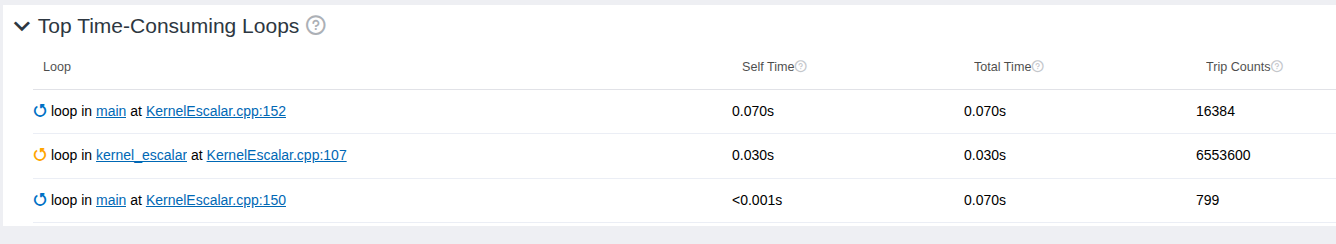
\includegraphics[width=\columnwidth]{timeLoops-Escalar}
\end{center}
\caption{Survey de bucles --- versi\'on Escalar. El kernel
(\texttt{kernel\_escalar:107}) reporta tipo \textit{Scalar}
con ISA SSE (uso escalar de registros XMM, sin SIMD empaquetado),
conforme al flag \texttt{-no-vec}. Trip count: 6{,}553{,}600.}
\label{fig:loops-escalar}
\end{figure}

\begin{figure}[htb]
\begin{center}
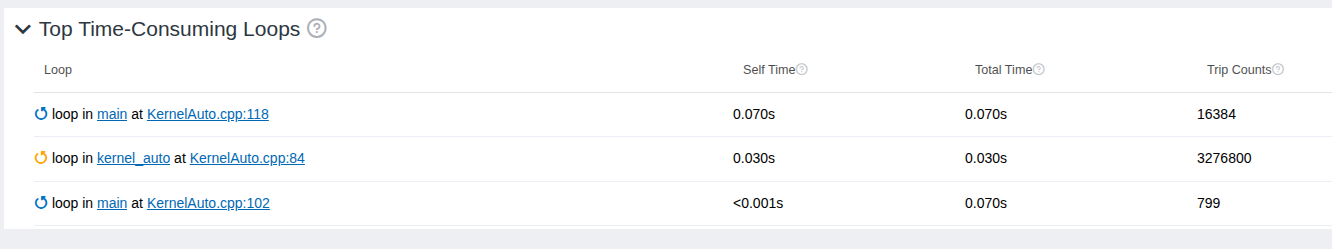
\includegraphics[width=\columnwidth]{timeLoops-Auto}
\end{center}
\caption{Survey de bucles --- versi\'on Autom\'atica. El kernel
(\texttt{kernel\_auto:84}) se marca como \textit{Vectorized (Body)}
con ISA AVX2 y trip count de 3{,}276{,}800, lo que corresponde
a un ancho vectorial de $52{,}428{,}800 / 3{,}276{,}800 = 16$
floats por iteraci\'on.}
\label{fig:loops-auto}
\end{figure}

\begin{figure}[htb]
\begin{center}
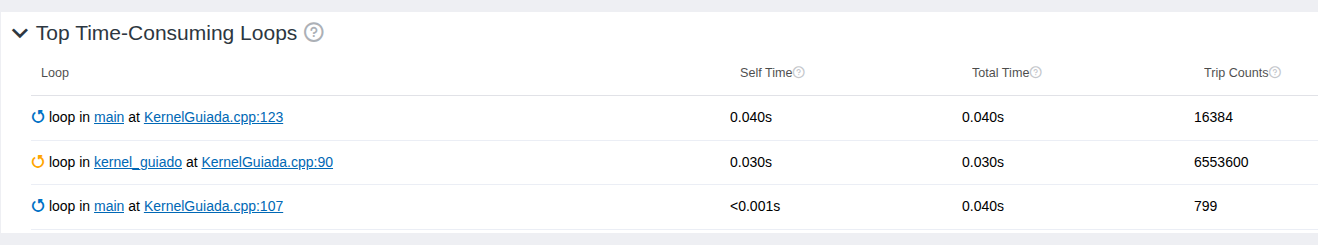
\includegraphics[width=\columnwidth]{timeLoops-Guiada}
\end{center}
\caption{Survey de bucles --- versi\'on Guiada. El kernel
(\texttt{kernel\_guiado:90}) aparece como \textit{Vectorized (Body)}
con ISA AVX2 y trip count de 6{,}553{,}600, correspondiente a un
ancho vectorial de~8 floats, exactamente el valor especificado
con \texttt{simdlen(8)}.}
\label{fig:loops-guiada}
\end{figure}

\begin{figure}[htb]
\begin{center}
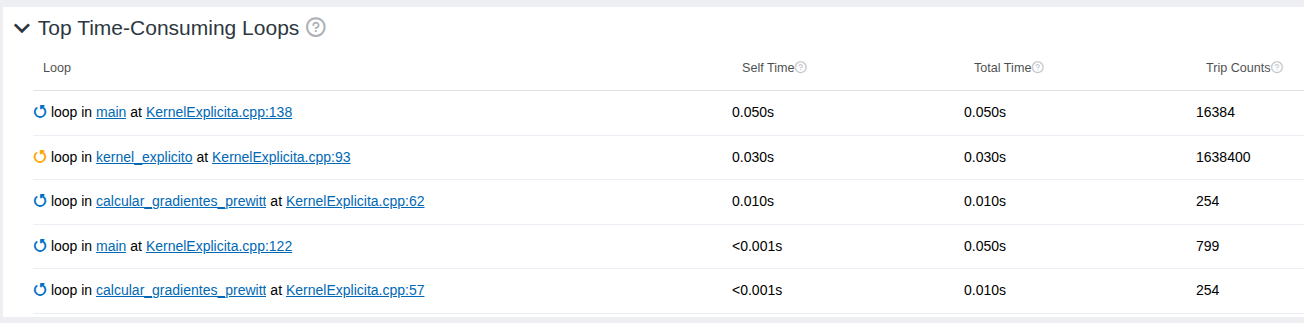
\includegraphics[width=\columnwidth]{timeLoops-Explicita}
\end{center}
\caption{Survey de bucles --- versi\'on Expl\'icita. El kernel
(\texttt{kernel\_explicito:93}) se reporta como \textit{Vectorized (Body)}
con ISA AVX2 y trip count de 1{,}638{,}400, lo que implica
un ancho efectivo de $52{,}428{,}800 / 1{,}638{,}400 = 32$
floats: el compilador aplic\'o adicionalmente un desenrollado
(\textit{unroll}) de $4\times$ sobre el bucle AVX2 escrito a mano.}
\label{fig:loops-explicita}
\end{figure}

La Tabla~\ref{tab:survey} resume los datos del Survey para los
kernels principales.

\begin{table}[htb]
\centering
\caption{Datos del Survey de Intel Advisor para el kernel Prewitt.}
\label{tab:survey}
\footnotesize
\begin{tabular}{@{}lcccc@{}}
\toprule
\textbf{Versi\'on} & \textbf{Tipo} & \textbf{ISA} &
\textbf{Trip count} & \textbf{Ancho vec.} \\
\midrule
Escalar     & Scalar           & SSE  & 6{,}553{,}600 & 1  \\
Autom\'atica & Vectorized (Body)& AVX2 & 3{,}276{,}800 & 16 \\
Guiada      & Vectorized (Body)& AVX2 & 6{,}553{,}600 &  8 \\
Expl\'icita  & Vectorized (Body)& AVX2 & 1{,}638{,}400 & 32$^*$ \\
\bottomrule
\multicolumn{5}{@{}l@{}}{\scriptsize $^*$ Incluye unroll $4\times$ aplicado por el compilador.}
\end{tabular}
\end{table}

\subsection{An\'alisis Roofline}

Las Figuras~\ref{fig:roofline-escalar} a~\ref{fig:roofline-explicita}
presentan el modelo Roofline generado por Intel Advisor para cada
versi\'on.

\begin{figure}[htb]
\begin{center}
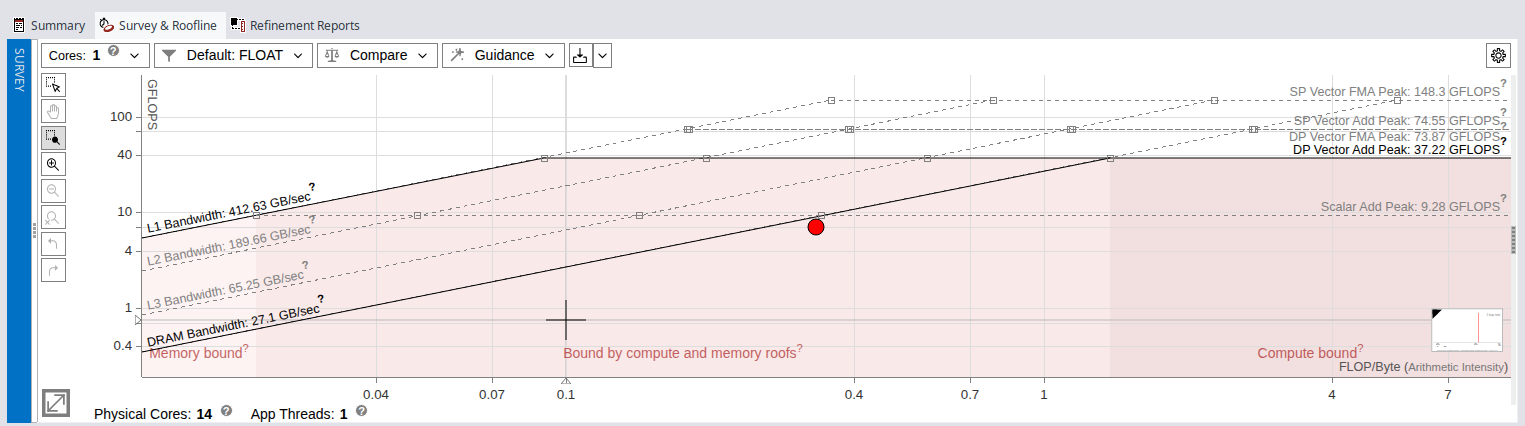
\includegraphics[width=\columnwidth]{graficaRoofline-Escalar}
\end{center}
\caption{Modelo Roofline --- versi\'on Escalar. El punto rojo
se ubica con AI $\approx 0.33$~FLOP/Byte y $\approx 6$--8~GFLOPS,
en la zona acotada entre los techos de ancho de banda L2/L3 y el
techo escalar (9.28~GFLOPS).}
\label{fig:roofline-escalar}
\end{figure}

\begin{figure}[htb]
\begin{center}
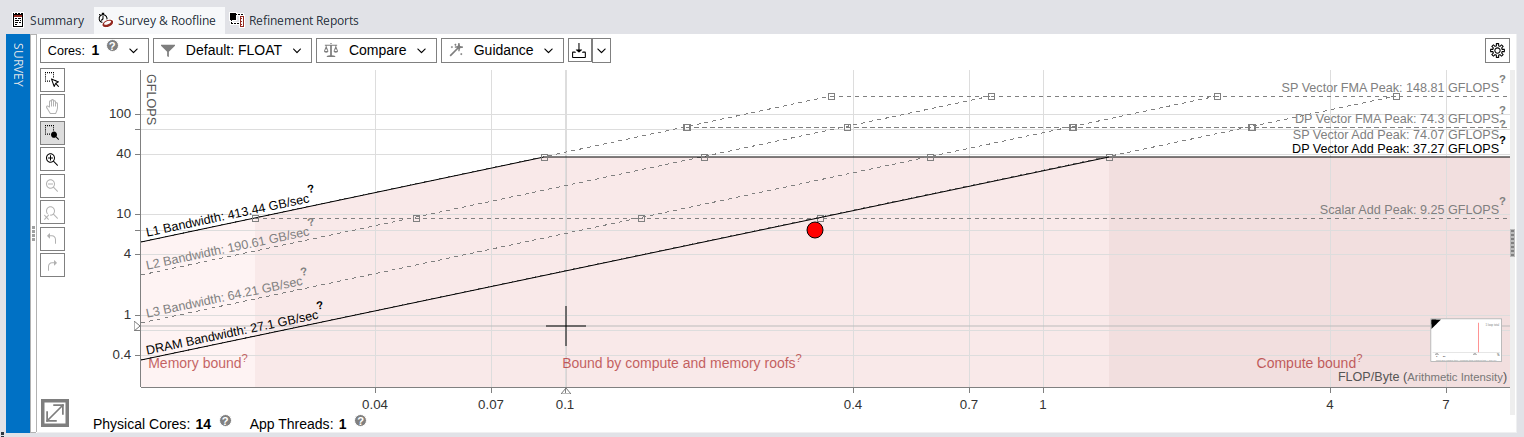
\includegraphics[width=\columnwidth]{graficaRoofline-Auto}
\end{center}
\caption{Modelo Roofline --- versi\'on Autom\'atica. El punto se
sit\'ua en la misma zona que el Escalar; la ganancia vectorial es
m\'inima porque la memoria no puede alimentar los registros AVX2
a la velocidad m\'axima.}
\label{fig:roofline-auto}
\end{figure}

\begin{figure}[htb]
\begin{center}
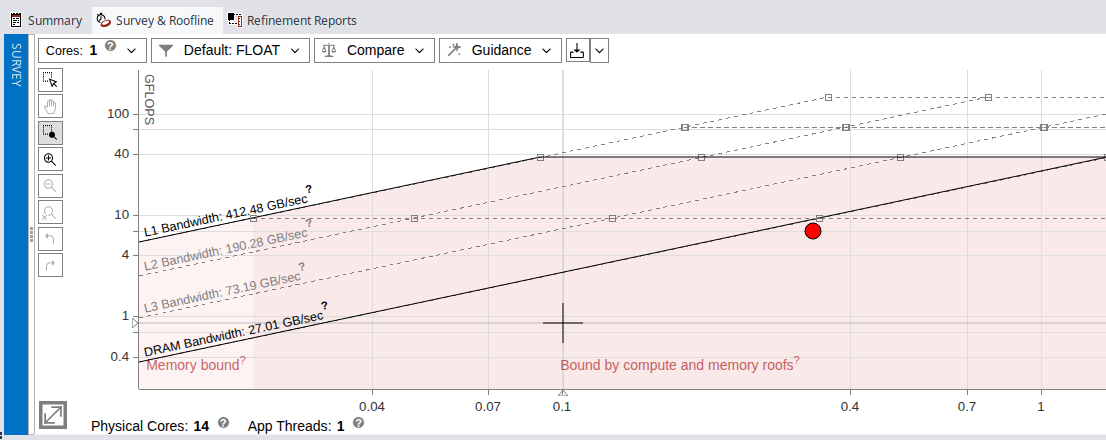
\includegraphics[width=\columnwidth]{graficaRoofline-Guiada}
\end{center}
\caption{Modelo Roofline --- versi\'on Guiada. Comportamiento
id\'entico a las versiones anteriores. El ancho vectorial de~8
(menor al de la versi\'on autom\'atica) resulta en rendimiento
similar al escalar.}
\label{fig:roofline-guiada}
\end{figure}

\begin{figure}[htb]
\begin{center}
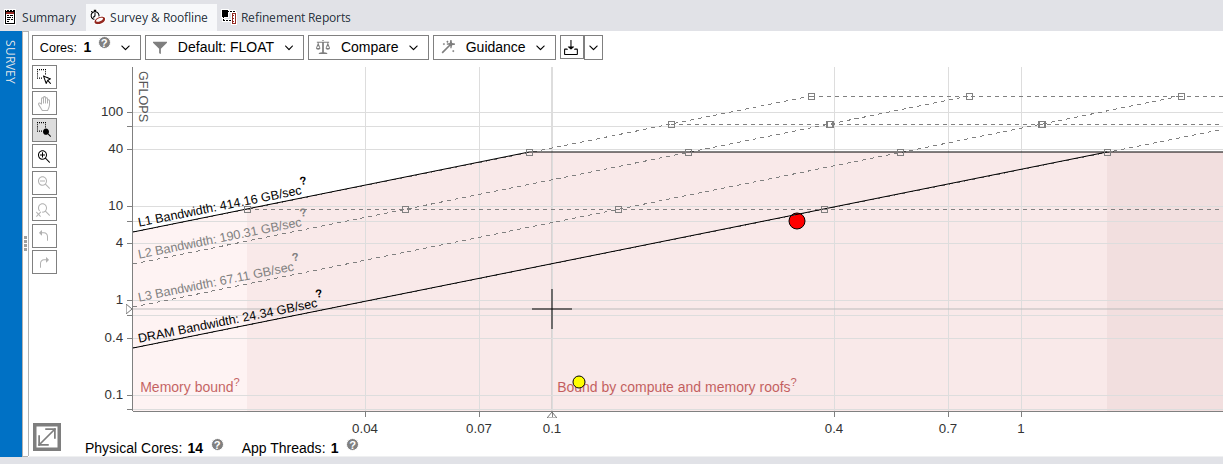
\includegraphics[width=\columnwidth]{graficaRoofline-Explicita}
\end{center}
\caption{Modelo Roofline --- versi\'on Expl\'icita. A pesar del
ancho efectivo de~32 floats (con unroll), el punto permanece en la
misma zona \textit{memory-bound}, con rendimiento ligeramente
superior al escalar.}
\label{fig:roofline-explicita}
\end{figure}

En los cuatro casos, el punto de operaci\'on se ubica en la regi\'on
denominada ``\textit{Bound by compute and memory roofs}'', a la
izquierda del punto de cresta del Roofline.
La intensidad aritm\'etica medida por Advisor para el programa
completo es de $\mathcal{I}_{\text{prog}} = 0.100$~FLOP/Byte,
inferior al valor te\'orico del kernel ($0.333$~FLOP/Byte),
porque Advisor incluye todas las operaciones de memoria del
programa (I/O de imagen PGM, c\'alculo de gradientes Prewitt,
replicaci\'on de datos), que diluyen la intensidad global.

\subsection{M\'etricas Generales del Programa}

Las Figuras~\ref{fig:metrics-escalar}
y~\ref{fig:metrics-auto} muestran los Program Metrics
reportados por Intel Advisor para las versiones Escalar y
Autom\'atica como versiones representativas.

\begin{figure}[htb]
\begin{center}
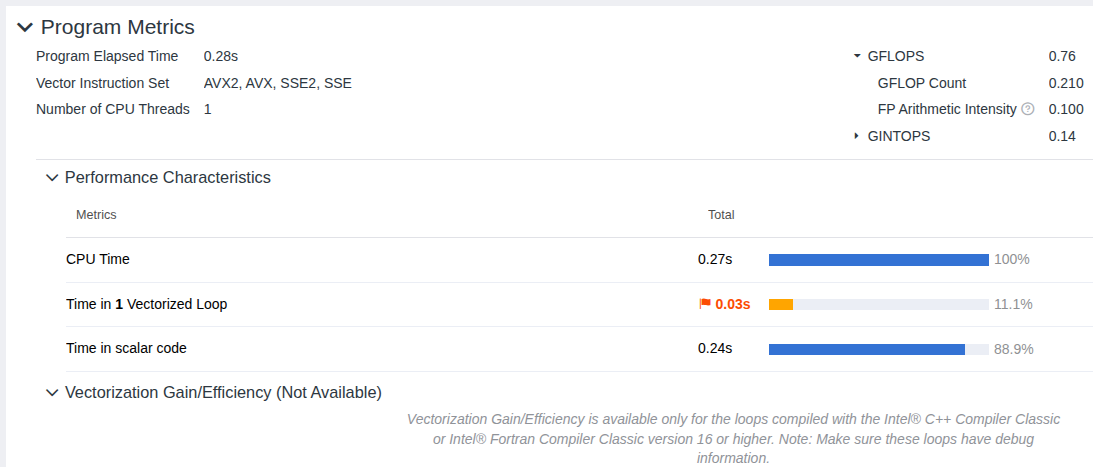
\includegraphics[width=\columnwidth]{summaryProgramMetrics-Escalar}
\end{center}
\caption{Program Metrics --- versi\'on Escalar. Tiempo total
$0.28$~s; rendimiento $0.76$~GFLOPS; tiempo del bucle vectorizado
(SSE escalar) $0.03$~s ($11\%$) frente a $0.24$~s ($89\%$) de
c\'odigo escalar (I/O, gradientes, replicaci\'on). ISA del
programa: AVX2, AVX, SSE2, SSE.}
\label{fig:metrics-escalar}
\end{figure}

\begin{figure}[htb]
\begin{center}
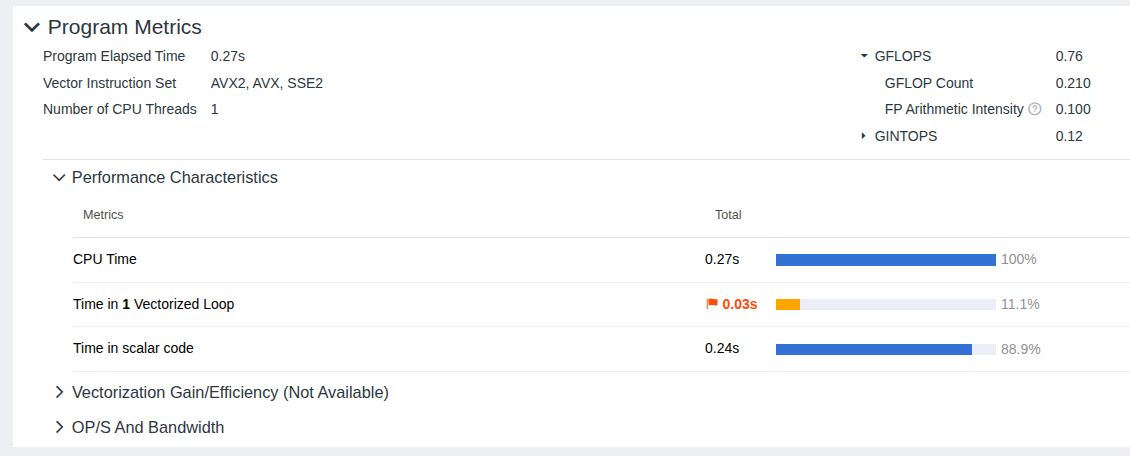
\includegraphics[width=\columnwidth]{summaryProgramMetrics-Auto}
\end{center}
\caption{Program Metrics --- versi\'on Autom\'atica. Tiempo total
$0.27$~s; rendimiento $0.76$~GFLOPS; tiempo del bucle AVX2
$0.03$~s ($11\%$). ISA del programa: AVX2, AVX, SSE2 (sin SSE
puro). La distribuci\'on de tiempos refleja que el kernel
vectorizado es solo una peque\~na fracci\'on del programa total.}
\label{fig:metrics-auto}
\end{figure}

La Tabla~\ref{tab:advisor-metricas} consolida los datos de
Program Metrics para las cuatro versiones.

\begin{table}[htb]
\centering
\caption{Resumen de m\'etricas de Intel Advisor (Program Metrics).}
\label{tab:advisor-metricas}
\footnotesize
\begin{tabular}{@{}lcccc@{}}
\toprule
\textbf{Versi\'on} & \textbf{Elapsed (s)} & \textbf{GFLOPS} &
\textbf{AI (FLOP/B)} & \textbf{Kernel (\%)} \\
\midrule
Escalar      & 0.28 & 0.76 & 0.100 & 11.1 \\
Autom\'atica  & 0.27 & 0.76 & 0.100 & 11.1 \\
Guiada       & 0.24 & 0.86 & 0.100 & 12.5 \\
Expl\'icita   & 0.26 & 0.82 & 0.100 & 12.0 \\
\bottomrule
\end{tabular}
\end{table}

Las Figuras~\ref{fig:metrics-guiada} y~\ref{fig:metrics-explicita}
complementan el panorama para las versiones Guiada y Expl\'icita.

\begin{figure}[htb]
\begin{center}
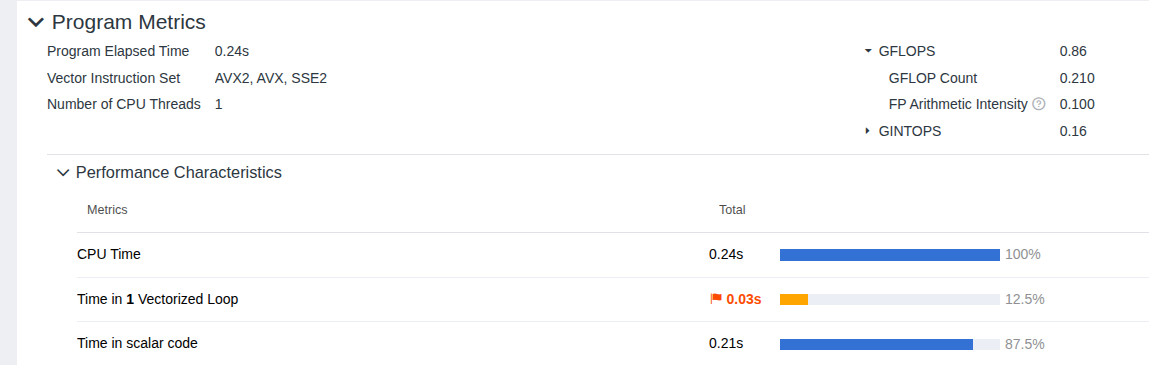
\includegraphics[width=\columnwidth]{summaryProgramMetrics-Guiada}
\end{center}
\caption{Program Metrics --- versi\'on Guiada. Tiempo total
$0.24$~s; rendimiento $0.86$~GFLOPS; bucle AVX2 con
\texttt{simdlen(8)} corresponde al $12.5\%$ del tiempo. Pese a
que el ancho vectorial es inferior al de la versi\'on autom\'atica,
el tiempo total es el menor de las cuatro, por variaciones de
timing en el c\'odigo escalar circundante.}
\label{fig:metrics-guiada}
\end{figure}

\begin{figure}[htb]
\begin{center}
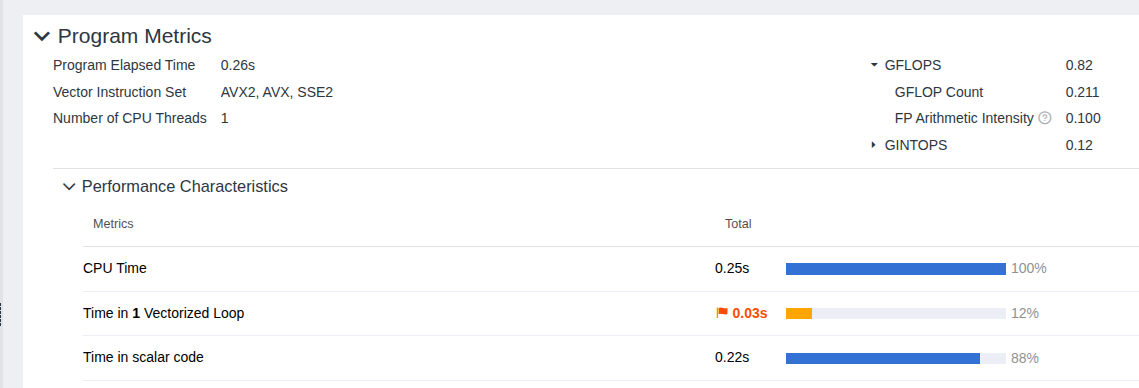
\includegraphics[width=\columnwidth]{summaryProgramMetrics-Explicita}
\end{center}
\caption{Program Metrics --- versi\'on Expl\'icita. Tiempo total
$0.26$~s; rendimiento $0.82$~GFLOPS; bucle AVX2 el $12\%$ del
tiempo. Dos bucles escalares adicionales de c\'alculo de gradientes
Prewitt (\texttt{calcular\_gradientes:57}, \texttt{:62}) son
visibles en el Survey de esta versi\'on; en las dem\'as no superan
el umbral de medici\'on de Advisor.}
\label{fig:metrics-explicita}
\end{figure}

Un hallazgo relevante es que el tiempo total del programa est\'a
dominado ($\approx 88$--$89\%$) por c\'odigo escalar: lectura de
la imagen PGM, c\'alculo de gradientes Prewitt con las m\'ascaras
3$\times$3, replicaci\'on de datos en memoria y escritura del
resultado.
El kernel vectorizado representa \'unicamente el $11$--$12\%$
del tiempo de ejecuci\'on total.
Esta distribuci\'on es independiente de la estrategia de
vectorizaci\'on empleada, ya que las partes escalares del
programa son las mismas en las cuatro versiones.

\subsection{An\'alisis de C\'odigo Activo (Code Analytics)}

El panel Code Analytics de Intel Advisor identifica las funciones
que mayor tiempo de c\'omputo consumen dentro de los bucles
vectorizados.
En las cuatro versiones, la funci\'on m\'as activa reportada es
\texttt{\_\_intel\_avx\_rep\_memset}, que es la rutina interna
del compilador para inicializaci\'on de memoria usando
instrucciones AVX.
Esto confirma que la mayor parte del tiempo vectorizado
corresponde a transferencias de datos en memoria y no a
operaciones aritm\'eticas, consistente con el car\'acter
\textit{memory-bound} revelado por el Roofline.

\begin{figure}[htb]
\begin{center}
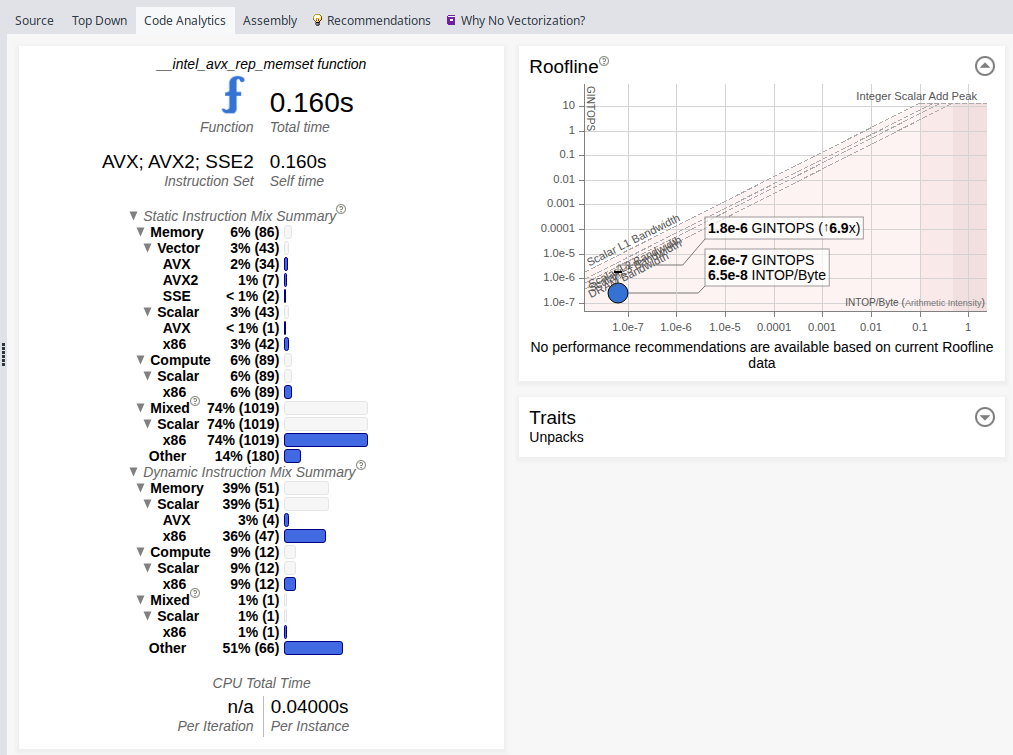
\includegraphics[width=\columnwidth]{codeAnalytics-Escalar}
\end{center}
\caption{Code Analytics --- versi\'on Escalar. El tiempo total
registrado en el bucle es de $0.16$~s, con un GINTOPS (giga
operaciones enteras por segundo) de speedup $6.9\times$ respecto
al techo escalar de referencia. La funci\'on dominante es
\texttt{\_\_intel\_avx\_rep\_memset}, lo que confirma que el
tiempo se gasta principalmente en movimiento de datos.}
\label{fig:analytics-escalar}
\end{figure}

\begin{figure}[htb]
\begin{center}
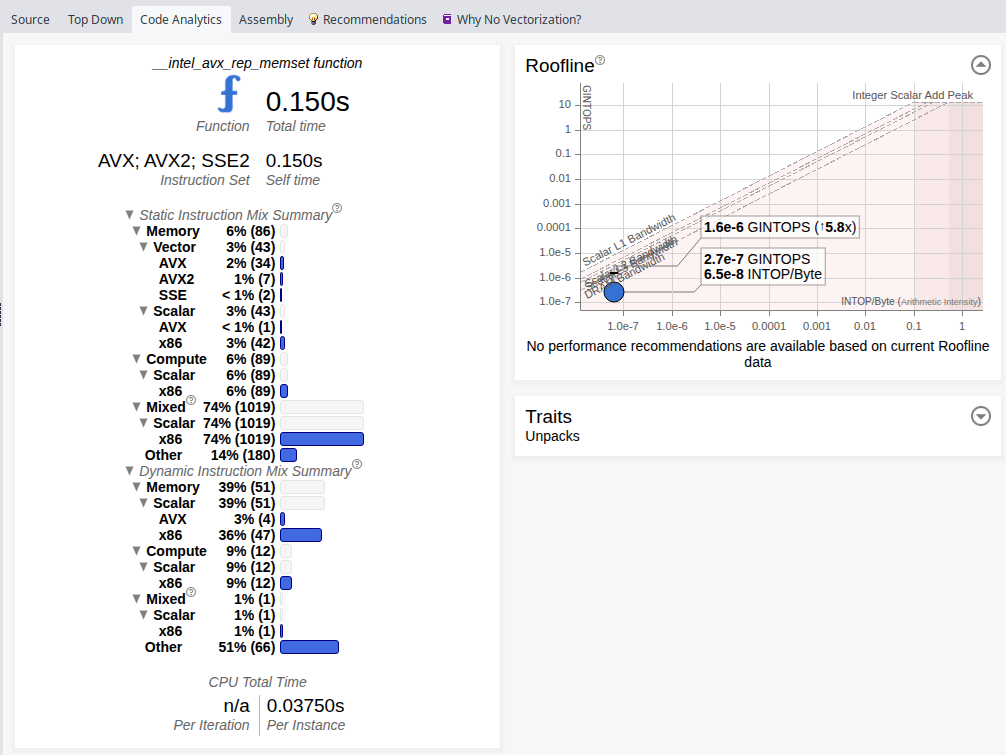
\includegraphics[width=\columnwidth]{codeAnalytics-Explicita}
\end{center}
\caption{Code Analytics --- versi\'on Expl\'icita. Tiempo de
$0.15$~s con speedup GINTOPS de $5.8\times$. Comparando con
la versi\'on Escalar ($6.9\times$), la diferencia en el perfil
de funciones activas confirma que los intr\'insecos AVX2
modifican el patr\'on de acceso a memoria respecto al c\'odigo
escalar, aunque ambas versiones siguen siendo dominadas por la
transferencia de datos.}
\label{fig:analytics-explicita}
\end{figure}

% =========================================================
%  SECCIÓN V — DISCUSIÓN
% =========================================================
\section{Discusi\'on}

\subsection{Comparaci\'on entre Versiones de Vectorizaci\'on}

Los resultados muestran que la vectorizaci\'on, aunque presente,
produce ganancias modestas sobre el kernel Prewitt en el hardware
utilizado.
La versi\'on autom\'atica es la que mejor rendimiento ofrece
($1.24\times$), seguida de la expl\'icita ($1.21\times$).
Resulta llamativo que la vectorizaci\'on guiada con
\texttt{simdlen(8)} no mejore significativamente sobre la escalar
($1.01\times$) pese a estar vectorizada con AVX2.

Este comportamiento se explica por el papel del ancho vectorial
real.
La versi\'on autom\'atica utiliza un ancho de~16~floats (AVX2
con posible unroll adicional), procesando el doble de datos por
iteraci\'on que la guiada (ancho~8).
La expl\'icita, aunque nominalmente de ancho~8, recibe un
desenrollado $4\times$ del compilador, resultando en un ancho
efectivo de~32, lo que tambi\'en supera a la guiada.
Sin embargo, todos estos anchos vectoriales son incapaces de
saturar el ancho de banda de memoria en igual medida que lo
har\'ian en un kernel de mayor intensidad aritm\'etica.

Desde la perspectiva de la complejidad de implementaci\'on:
\begin{itemize}
  \item La \textbf{autom\'atica} requiere el menor esfuerzo y
    produce el mejor resultado; solo necesita compilar con
    \texttt{-O3 -march=native} y usar \texttt{\_\_restrict}.
  \item La \textbf{guiada} requiere conocer el pragma de OpenMP
    SIMD y elegir el \texttt{simdlen} adecuado; result\'o inferior
    porque \texttt{simdlen(8)} es m\'as conservador que la
    decisi\'on autom\'atica del compilador.
  \item La \textbf{expl\'icita} requiere dominar los intr\'insecos
    AVX2 y resulta en rendimiento ligeramente menor que la
    autom\'atica, mostrando que el compilador tambi\'en puede
    optimizar el c\'odigo escalar mejor que la versi\'on manual
    de ancho~8 sin unroll.
\end{itemize}

\subsection{Interpretaci\'on del Modelo Roofline}

La intensidad aritm\'etica te\'orica del kernel es
$\mathcal{I} = 0.333$ FLOP/Byte (ec.~\ref{eq:ai}).
Este valor sit\'ua el kernel \textit{por debajo} del punto de
cresta del Roofline calculado como:

\begin{equation}
  \mathcal{I}_{\text{cresta}} =
  \frac{P_{\text{peak}}}{B_{\text{mem}}} \approx
  \frac{9.28 \text{ GFLOPS}}{24 \text{ GB/s}} \approx
  0.387 \text{ FLOP/Byte}
\end{equation}

Al ser $\mathcal{I} = 0.333 < \mathcal{I}_{\text{cresta}} = 0.387$,
el kernel es \textbf{memory-bound}: el cuello de botella es el
ancho de banda de memoria, no la capacidad de c\'omputo.
Esto significa que aunque se utilicen instrucciones AVX2 de
m\'axima eficiencia, los registros YMM permanecer\'an ociosos
una parte del tiempo esperando que la memoria entregue los datos.

El techo alcanzable con la memoria DRAM a $24$~GB/s ser\'ia:
\begin{equation}
  P_{\max}^{\text{DRAM}} = 0.333 \times 24 \approx 8.0 \text{ GFLOPS}
\end{equation}

Los resultados experimentales (5.92--7.34~GFLOPS) son coherentes
con este l\'imite te\'orico, confirmando que el kernel opera
pr\'oxima a la banda de datos de la jerarqu\'ia de cach\'e
L2/L3 del procesador ($65$--$190$~GB/s) m\'as que de la DRAM,
lo que explica que los GFLOPS medidos superen el techo DRAM.

\subsection{ISA Detectada por Versi\'on}

Intel Advisor reporta la ISA (\textit{Instruction Set Architecture})
utilizada en cada programa:

\begin{itemize}
  \item \textbf{Escalar}: AVX2, AVX, SSE2, \textbf{SSE}.
    La presencia de instrucciones SSE puras (sin empaquetado)
    confirma que el kernel usa registros XMM en modo escalar
    (un solo float por registro), no SIMD empaquetado.
    El flag \texttt{-no-vec} proh\'ibe el uso vectorial, pero
    el procesador sigue usando los registros SSE para operaciones
    escalares.

  \item \textbf{Autom\'atica}: AVX2, AVX, SSE2 (sin SSE puro).
    La ausencia de SSE puro confirma que el kernel escal\'o al
    modo AVX2 empaquetado.

  \item \textbf{Guiada}: AVX2, AVX, SSE2 (sin SSE puro).
    Idéntico al autom\'atico en cuanto a ISA, aunque con ancho~8
    en vez de~16.

  \item \textbf{Expl\'icita}: AVX2, AVX, SSE2 (sin SSE puro).
    Los intr\'insecos \texttt{\_mm256\_*} garantizan el uso de
    registros YMM de 256~bits.
\end{itemize}

\subsection{Dominancia del C\'odigo Escalar y Ley de Amdahl}

Un resultado relevante es que el bucle de replicaci\'on de
datos (el que extiende la imagen 800 veces en memoria para
alcanzar $N_{\text{tot}}$) consume entre $0.040$ y $0.070$~s,
superando al propio kernel vectorizado ($0.030$~s).
Esto implica que la mayor parte del tiempo lo ocupan operaciones
fuera del kernel: lectura del archivo PGM, c\'alculo de los
gradientes Prewitt con las m\'ascaras $3\times3$ (bucle escalar
de 254 iteraciones), replicaci\'on de datos y escritura
del resultado.

Este comportamiento puede analizarse formalmente con la
\textbf{Ley de Amdahl}~\cite{sutter2005}.
Sea $p$ la fracci\'on paralelizable del programa y $f$ el
factor de aceleraci\'on (\textit{speedup}) de esa fracci\'on.
El speedup total del programa est\'a acotado por:

\begin{equation}
  S(f) = \frac{1}{(1-p) + p/f}
  \label{eq:amdahl}
\end{equation}

En nuestro caso, $p \approx 0.12$ (el kernel representa el
$12\%$ del tiempo total) y $1-p \approx 0.88$ es la fracci\'on
escalar fija.
La Tabla~\ref{tab:amdahl} muestra el speedup total m\'aximo
te\'orico en funci\'on del factor $f$ del kernel:

\begin{table}[htb]
\centering
\caption{Speedup m\'aximo total predicho por la Ley de Amdahl
($p=0.12$, $1-p=0.88$).}
\label{tab:amdahl}
\footnotesize
\begin{tabular}{@{}ccc@{}}
\toprule
\textbf{Speedup kernel} $f$ & \textbf{Speedup total} $S(f)$ &
\textbf{Mejora (\%)} \\
\midrule
$1\times$ (escalar)  & 1.00 &  ---  \\
$2\times$            & 1.09 &  +9\% \\
$4\times$            & 1.11 & +11\% \\
$8\times$  (AVX2 t.) & 1.12 & +12\% \\
$16\times$ (AVX2 m.) & 1.12 & +12\% \\
$\infty$             & 1.14 & +14\% \\
\bottomrule
\end{tabular}
\end{table}

El speedup te\'orico m\'aximo posible, incluso vectorizando el
kernel infinitamente r\'apido, es de apenas $1.14\times$.
Los speedups experimentales observados ($1.01$--$1.24\times$)
son consistentes con este l\'imite te\'orico, validando que
el dise\~no del experimento es correcto.
La \'unica forma de superar este techo ser\'ia vectorizar
tambi\'en las partes escalares del programa (c\'alculo de
gradientes, replicaci\'on de datos).

\subsection{Limitaciones y Trabajo Futuro}

La m\'etrica \textit{Vectorization Gain/Efficiency} de Intel
Advisor reporta \textit{Not Available} en todas las versiones.
Esto se debe a que dicha m\'etrica requiere el compilador Intel
C++ cl\'asico (\texttt{icc}/\texttt{icpc} versi\'on 16+), y el
presente trabajo utiliz\'o \texttt{icpx} (compilador DPC++ de
la generaci\'on oneAPI).
Para trabajo futuro se recomienda explorar:
(a)~operadores de mayor intensidad aritm\'etica como el filtro
Gaussiano o la convolución 2D densa, que ser\'ian m\'as
sensibles a la vectorizaci\'on;
(b)~an\'alisis multi-hilo con OpenMP para aprovechar los
14~n\'ucleos disponibles;
(c)~uso de AVX-512 si el hardware lo soporta, para alcanzar
anchos de~16 o~32 floats con mayor eficiencia que el unroll.

% =========================================================
%  SECCIÓN VI — CONCLUSIONES
% =========================================================
\section{Conclusiones}

Este trabajo present\'o el an\'alisis comparativo de cuatro
estrategias de vectorizaci\'on SIMD aplicadas al kernel num\'erico
del operador Prewitt para detecci\'on de bordes en im\'agenes.
A partir de los resultados obtenidos se establecen las siguientes
conclusiones:

\begin{enumerate}
  \item \textbf{El kernel Prewitt es memory-bound.}
    Su intensidad aritm\'etica te\'orica de $0.333$~FLOP/Byte
    lo coloca a la izquierda del punto de cresta del modelo
    Roofline ($0.387$~FLOP/Byte), lo que significa que el
    cuello de botella de rendimiento es el ancho de banda de
    memoria y no la capacidad de c\'omputo del procesador.
    Esta conclusi\'on es independiente del nivel de vectorizaci\'on
    aplicado y fue confirmada por las cuatro gr\'aficas Roofline
    generadas con Intel Advisor.

  \item \textbf{La vectorizaci\'on produce ganancias modestas.}
    El speedup m\'aximo observado fue de $1.24\times$ para la
    vectorizaci\'on autom\'atica y de $1.21\times$ para la
    expl\'icita.
    En un kernel \textit{compute-bound}, estos mismos anchos
    vectoriales (16$\times$ y 32$\times$ efectivo) producir\'ian
    speedups proporcionales al ancho SIMD.
    La modestia de los resultados es, por tanto, esperada y
    correcta dado el car\'acter \textit{memory-bound} del kernel.

  \item \textbf{La vectorizaci\'on autom\'atica es la m\'as eficiente.}
    El compilador \texttt{icpx} con \texttt{-O3 -march=native}
    elige un ancho vectorial de~16~floats y genera instrucciones
    AVX2 \'optimas sin intervenci\'on del programador, superando
    incluso a la versi\'on expl\'icita en t\'erminos de relaci\'on
    rendimiento-esfuerzo.
    Esto subraya el alto nivel de madurez de los optimizadores
    modernos de compiladores Intel.

  \item \textbf{La vectorizaci\'on guiada requiere ajuste del simdlen.}
    El pragma \texttt{simdlen(8)} impuso un ancho menor al
    elegido autom\'aticamente por el compilador, resultando en
    rendimiento pr\'acticamente igual al escalar.
    Una elecci\'on de \texttt{simdlen(16)} o dejando que el
    compilador decida habr\'ia producido mejores resultados.

  \item \textbf{El 88\% del programa es c\'odigo escalar.}
    La fracci\'on vectorizable del programa (el kernel) representa
    solo el 11--12\% del tiempo total de ejecuci\'on.
    El tiempo dominante corresponde a operaciones inherentemente
    escalares: lectura/escritura de archivos PGM, c\'alculo
    de gradientes 2D con m\'ascaras 3$\times$3, y replicaci\'on
    de datos en memoria.
    Esta distribuci\'on limita el speedup global del programa de
    acuerdo con la Ley de Amdahl.

  \item \textbf{Intel Advisor es una herramienta diagn\'ostica
    valiosa.}
    El Survey, los trip counts y el modelo Roofline permitieron
    confirmar objetivamente el ancho vectorial real de cada
    versi\'on, identificar el cuello de botella de memoria y
    cuantificar la fracci\'on vectorizable del programa.
    Su integraci\'on en el flujo de desarrollo es recomendable
    para cualquier proyecto de optimizaci\'on de kernels HPC.
\end{enumerate}

\section*{Agradecimientos}

El autor agradece al Dr.~Mario Rossainz L\'opez, profesor del
curso de Programaci\'on en Plataformas Multicore de la Benem\'erita
Universidad Aut\'onoma de Puebla (BUAP), por el dise\~no de la
actividad y la gu\'ia metodol\'ogica que permitieron llevar a cabo
este trabajo de manera rig\'urosa.


% =========================================================
%  BIBLIOGRAFIA
% =========================================================
\bibliographystyle{Jornadas}
\bibliography{biblio}

\end{document}
